% !TEX root = ../SU2-Scitech15.tex

\subsection*{Reynolds-averaged Navier-Stokes (RANS) equations}
We are concerned with time-accurate, viscous flow around aerodynamic bodies in arbitrary motion which is governed by the compressible, unsteady Navier-Stokes equations. Consider the equations in a domain, $\Omega \subset \mathbb{R}^3 $, with a disconnected boundary that is divided into a far-field component, $\Gamma_\infty$, and an adiabatic wall boundary, $S$, as seen in Fig.~\ref{domain}. The surface $S$ represents the outer mold line of an aerodynamic body, and it is considered continuously differentiable ($C^1$). These conservation equations along with a generic source term, $\mathcal{Q}$, can be expressed in an arbitrary Lagrangian-Eulerian (ALE)~\cite{donea2004} differential form as
\begin{equation} \label{rans}
\left\{\begin{array} {lll}
\mathcal{R}(U) = \frac{\partial U}{\partial t} + \nabla \cdot \vec{F}^{c}_{ale} -  \nabla \cdot \vec{F}^{v} - \mathcal{Q} = 0 & \mbox{  in } \Omega, & t > 0  \\
\vec{v} = \vec{u}_\Omega &  \mbox{ on }  S,  \\
\partial_n T = 0 &  \mbox{ on }  S,   \\
(W)_+ = W_\infty  & \mbox{ on }  \Gamma_\infty, \\
\end{array}\right.
\end{equation}
where the conservative variables are given by $U = \left \{  \rho, \rho \vec{v},  \rho E \right \}^\mathsf{T}$, and the convective fluxes, viscous fluxes, and source term are
\begin{align} \label{fluxes}
\vec{F}^{c}_{ale} = \left \{ \begin{array}{c} \rho (\vec{v} - \vec{u}_\Omega)  \\ \rho \vec{v} \otimes  (\vec{v} - \vec{u}_\Omega) + \bar{\bar{I}} p \\ \rho E (\vec{v} - \vec{u}_\Omega) + p \vec{v}   \end{array} \right \},  ~ ~ ~
\vec{F}^{v} = \left \{ \begin{array}{c} \cdot \\ \bar{\bar{\tau}} \\ \bar{\bar{\tau}} \cdot \vec{v}  + \mu_{tot}^* c_p \nabla T\end{array} \right  \},  ~ ~ ~
\mathcal{Q} = \left \{ \begin{array}{c} q_{\rho} \\ \vec{q}_{\rho \vec{v}} \\ \ q_{\rho E}   \end{array} \right \}, 
\end{align} 
where $\rho$ is the fluid density, $\vec{v} = \{v_1, v_2, v_3\}^\mathsf{T} \in \mathbb{R}^{3}$ is the flow speed in a Cartesian system of reference, $\vec{u}_\Omega$ is the velocity of a moving domain (mesh velocity after discretization), $E$ is the total energy per unit mass, $p$ is the static pressure, $c_p$ is the specific heat at constant pressure, $T$ is the temperature, and the viscous stress tensor can be written in vector notation as
\begin{align} \label{tau}
\bar{\bar{\tau}} = \mu _{tot} \left(\nabla \vec{v} + {\nabla \vec{v}}^\mathsf{T}  - \frac{2}{3} \bar{\bar{I}} (\nabla \cdot \vec{v} )\right).
\end{align}
\begin{wrapfigure}{r}{0.4\linewidth}
  \begin{center}
   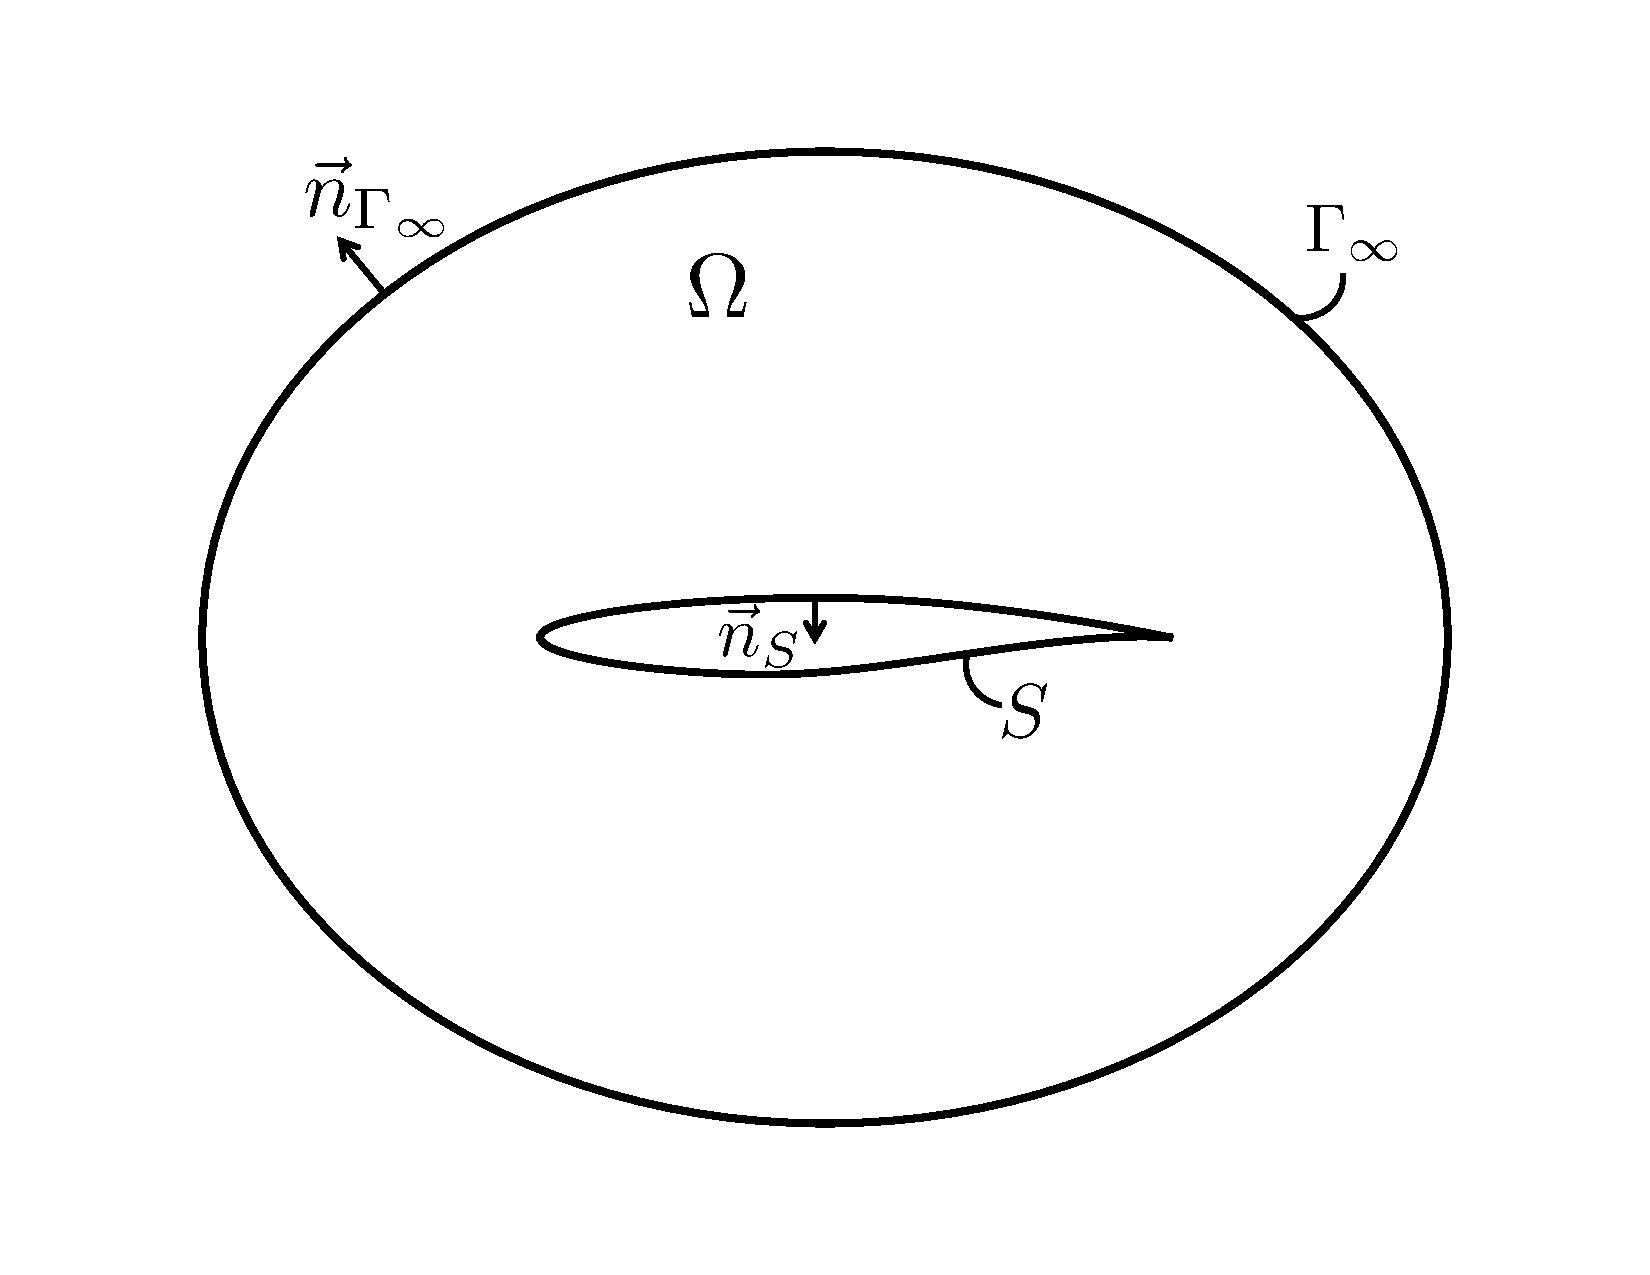
\includegraphics[width=2.4in]{domain.pdf}
    \caption{Notional schematic of the flow domain, $\Omega$, the boundaries, $\Gamma_\infty$ and $S$, as well as the definition of the surface normals.}
    \label{domain}
  \end{center}
\end{wrapfigure}
The second line of Eqn.~\ref{rans} represents the no-slip condition at a solid wall, the third line represents an adiabatic condition at the wall, and the final line represents a characteristic-based boundary condition at the far-field~\cite{hirsch1984} with $W$ representing the characteristic variables. 

Note that the boundary conditions also take into account any domain motion, but for problems on fixed grids ($\vec{u}_\Omega = 0$), Eqn.~\ref{rans} reduces to a purely Eulerian formulation.  We will use the free-stream fluid state as the initial condition for the mean flow for all simulations run.

Assuming a perfect gas with a ratio of specific heats, $\gamma$, and gas constant, $R$, the pressure is determined from $p = (\gamma-1) \rho \left [ E - 0.5(\vec{v} \cdot \vec{v} ) \right ]$, the temperature is given by $T = p/(\rho R)$, and $c_p= \gamma R/(\gamma - 1)$. In accord with the standard approach to turbulence modeling based upon the Boussinesq hypothesis~\cite{wilcox98}, which states that the effect of turbulence can be represented as an increased viscosity, the total viscosity is divided into a laminar, $\mu _{dyn}$, and a turbulent, $\mu _{tur}$, component. In order to close the system of equations, the dynamic viscosity, $\mu _{dyn}$, is assumed to satisfy Sutherland's law~\cite{White1974} (function of temperature alone), the turbulent viscosity $\mu_{tur}$ is computed via a turbulence model, and
\begin{equation}
\label{eq:viscosities}
\mu _{tot}=\mu _{dyn}+\mu _{tur}, \quad
\mu _{tot}^*=\frac{\mu _{dyn}}{Pr_{d}}+\frac{\mu _{tur}}{Pr_{t}},
\end{equation}
where $Pr_{d}$ and $Pr_{t}$ are the dynamic and turbulent Prandtl numbers, respectively.  The turbulent viscosity, $\mu_{tur}$, is obtained from the Spalart-Allmaras (S-A) model involving the flow state and a set of new variables. 

\subsection*{Spalart-Allmaras Turbulence model}
In the case of the one-equation Spalart-Allmaras~\cite{spalart1992} turbulence model, the turbulent viscosity is computed as
\begin{equation} \label{eq nutur}
\mu _{tur}=\rho \hat{\nu}f_{v1},\quad f_{v1}=\frac{\chi ^{3}}{\chi ^{3}+c_{v1}^{3}}\mbox{,}\quad \chi =\frac{%
\hat{\nu}}{\nu }\mbox{,}\quad \nu =\frac{\mu _{dyn}}{\rho }.
\end{equation}
The new variable $\hat \nu$ is obtained by solving a transport equation where the convective, viscous, and source terms are given as follows:
\begin{equation} \label{eq:tersa0}
\vec F^{c} =  \vec v\hat{\nu},\quad
\vec F^{v} =  - \frac{\nu +\hat{\nu}}{\sigma }\nabla\hat{\nu},\quad
Q =  c_{b1}\hat{S}\hat{\nu}-c_{w1}f_{w}\left( \frac{\hat{\nu}}{d_{S}}\right) ^{2}+\frac{c_{b2}}{\sigma } |\nabla \hat{\nu}|^{2},
\end{equation}
where the production term $\hat S$ is defined as $\hat{S} = |\vec \omega| +\frac{\hat{\nu}}{\kappa ^{2}d_{S}^{2}}f_{v2}$ , $\vec \omega= \nabla \times \vec v$ is the fluid vorticity, $d_{S}$ is the distance to the nearest wall, and $f_{v2}=1-\frac{\chi }{1+\chi f_{v1}}$. The function $f_{w}$ is computed as $f_{w}=g\left[ \frac{1+c_{w3}^{6}}{g^{6}+c_{w3}^{6}}\right] ^{1/6}$, where $g=r+c_{w2}(r^{6}-r)$ and $r=\frac{\hat{\nu}}{\hat{S}\kappa ^{2}d_{S}^{2}}$. Finally, the set of closure constants for the model is given by 
\begin{equation}
\sigma =2/3,\;  c_{b1}=0.1355,\; c_{b2}=0.622,\; \kappa =0.41, \;c_{w1}=\frac{c_{b1}}{\kappa^2}+\frac{1+c_{b2}}{\sigma}, \; c_{w2}=0.3, \; c_{w3}=2, \; c_{v1}=7.1. 
\end{equation}

The physical meaning of the far-field boundary condition for the turbulent viscosity is the imposition of some fraction of the laminar viscosity at the far-field. On viscous walls, $\hat{\nu}$ is set to zero, corresponding to the absence of turbulent eddies very near to the wall.

